\documentclass[12pt, a4paper]{article}

\usepackage[export]{adjustbox}
\usepackage{fancyhdr}
\usepackage[utf8]{inputenc}
\usepackage[english]{babel}
\usepackage{longtable}
\usepackage[margin=2cm, bottom=4cm]{geometry}
\usepackage{color,soul}
\usepackage{booktabs}
\usepackage{pdfpages}

\pagestyle{fancy}
\fancyhf{}% Clear all headers/footers
\renewcommand{\headrulewidth}{.4pt}% Header rule width
\renewcommand{\footrulewidth}{0pt}% No footer rule
\fancyhead[L]{% Left header
  \rule[-1\baselineskip]{0pt}{0pt}% Strut to ensure a 1/4 \baselineskip between image and header rule
  
\includegraphics[height=2\baselineskip,valign=c]{figures/logo_MRS_short_bw.png}% Image
  \quad% Space
}


\fancyhead[R]{
MRS MODULE HOST
}

\chead{\thepage}


\title{
\Huge{MRS MODULE HOST}\\
{REVISION 1}\\
\vspace{0.5cm}
\LARGE{David Zaitlik}\\
\vspace{0.5cm}
\normalsize{\textit{Multi-Robot Systems Group, FEE CTU in Prague}}\\
\vspace{1.5cm}
\vfill
\begin{figure}[h]
\centering

\includegraphics[width=\textwidth]{figures/logo_CTU_FEE_MRS_blue.png}
\end{figure}
\date{\today}

}

\setlength{\headheight}{3.5\baselineskip}% To accommodate new oversized header



\begin{document}
\clearpage
\maketitle
\thispagestyle{empty}

\pagebreak
\tableofcontents
\listoffigures
\listoftables
\thispagestyle{empty}

\pagebreak
\setcounter{page}{1}
\pagenumbering{arabic}
\section{Introduction}
MRS Modules are designed to be powered by a drone power supply and to communicate with an Intel NUC onboard computer. However, it is inconvenient to have it plugged into a drone for development and testing. Therefore this Host Board was designed.\\
\\
This board contains a single UART to USB converter to provide communication between the module's MCU and the developer's laptop.\\
\\
The 5V is supplied directly from USB, and the "battery voltage" can be provided using the barrel connector and an external power supply.

\begin{figure}[h]
\centering
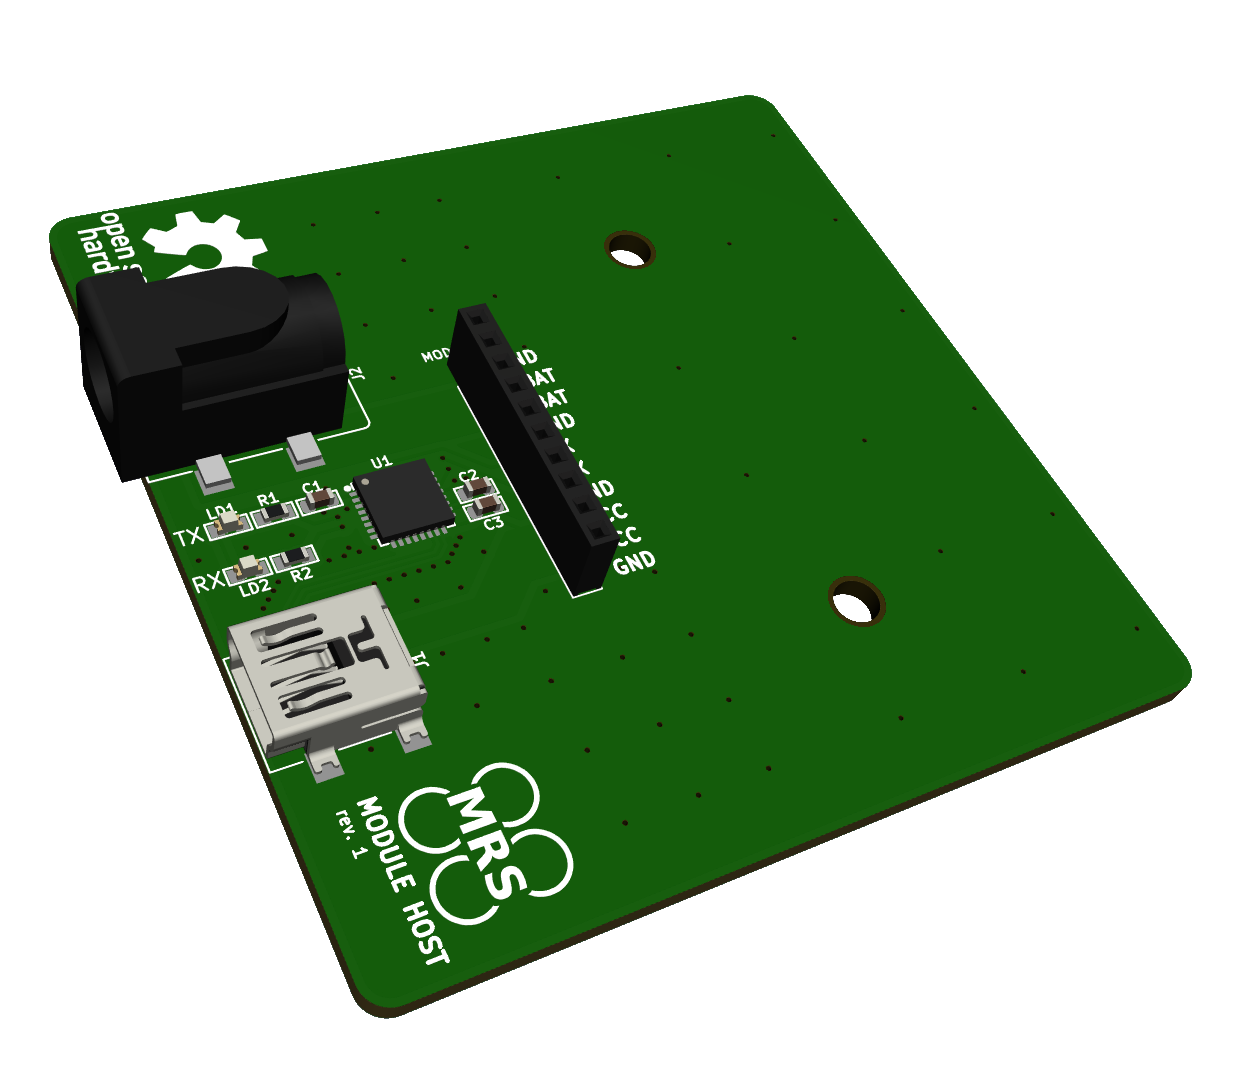
\includegraphics[width=0.9\textwidth]{figures/Thumbnail.png}
\caption{MRS MODULE HOST: Thumbnail}
\label{fig:thumbnail}
\end{figure}

\pagebreak
\section{Dimensions}
The board is 60mm wide and 60mm long with mounting holes for an MRS module.

The mechanical drawing can be seen in Figure \ref{fig:dimensions} below.

\begin{figure}[h]
\centering
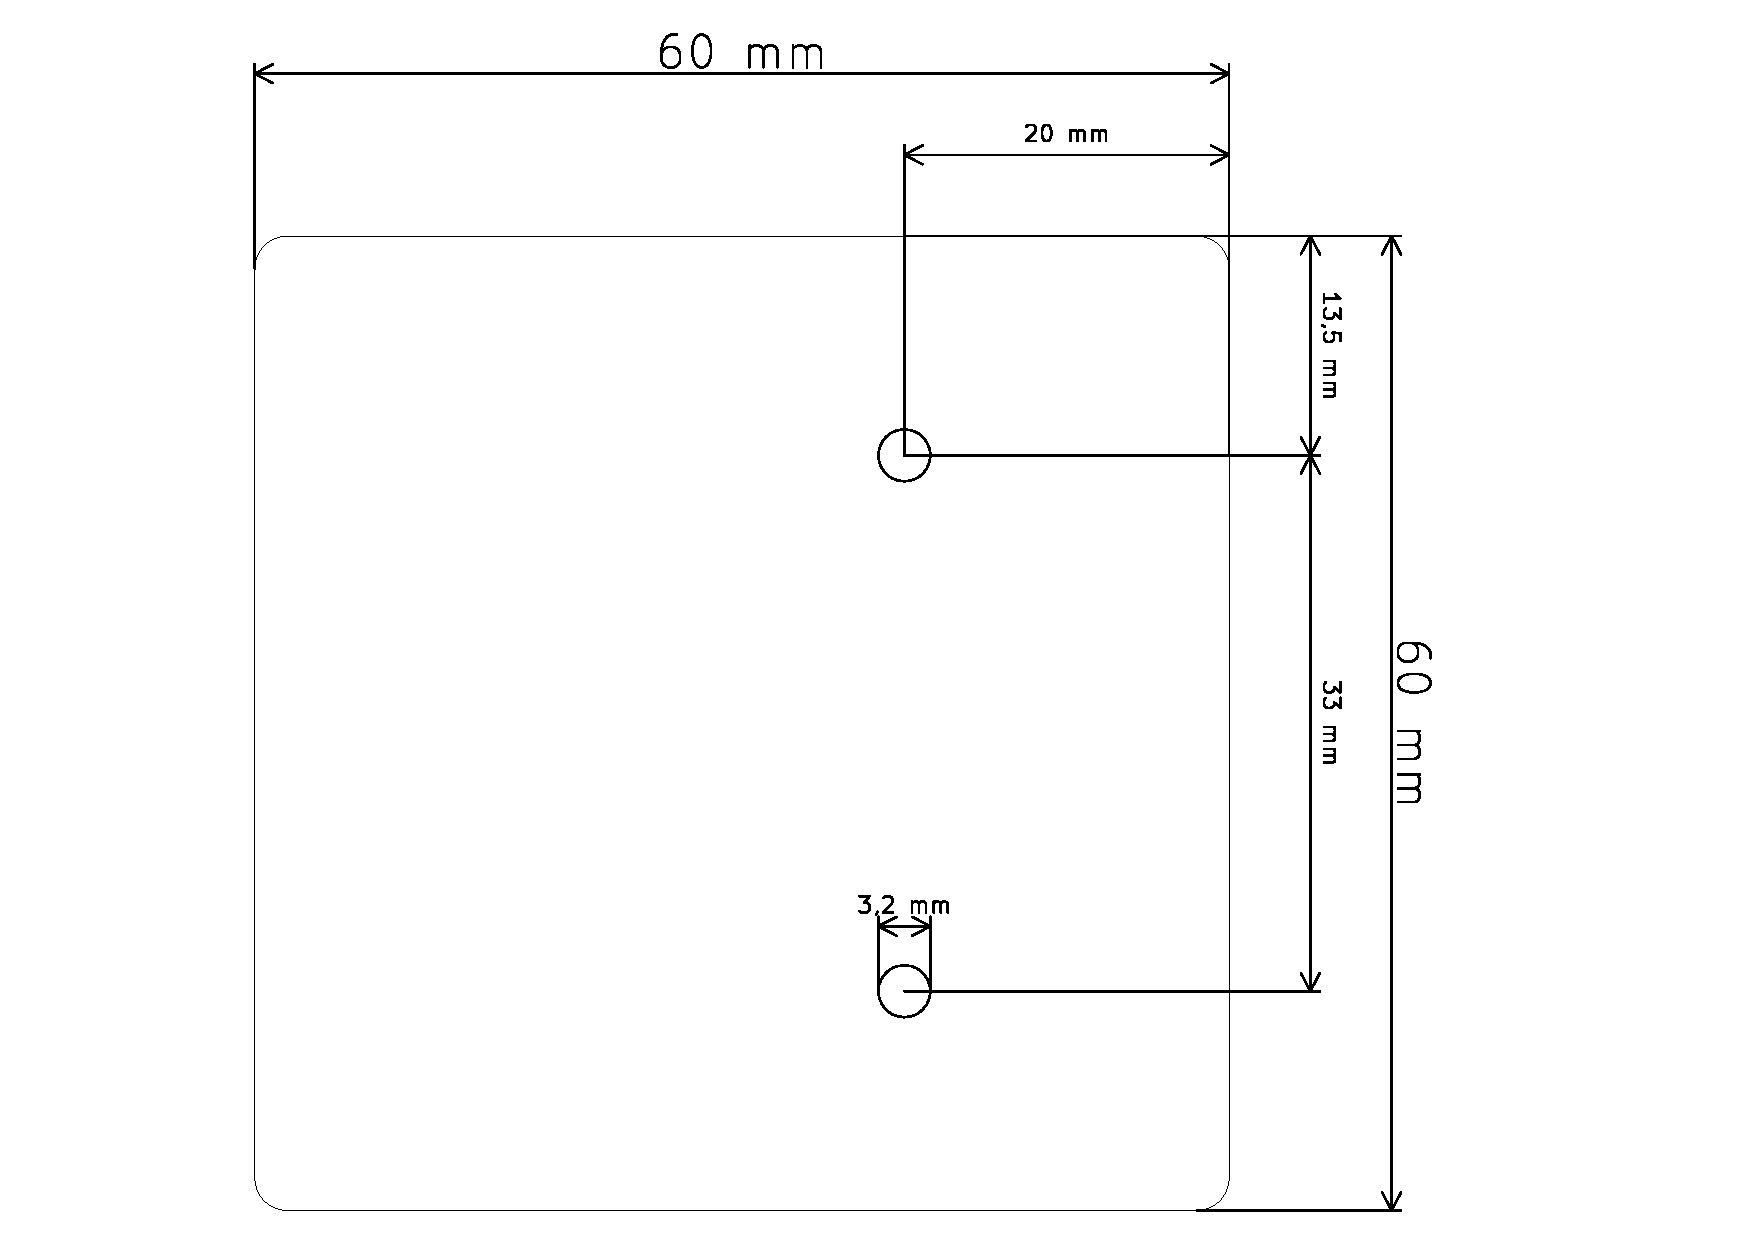
\includegraphics[width=\textwidth]{figures/Dimensions.pdf}
\caption{MRS MODULE HOST: Dimensions}
\label{fig:dimensions}
\end{figure}

\pagebreak
\section{Connectors}
The Module Host Board has connectors only on the top layer.
The connector marked as \verb|USB B MINI| is a standard USB B Mini connector. It provides connectivity between the user's computer and an MRS Module's MCU using an FTDI IC and 5V for the module.\\
\\
The connector marked as \verb|POWER (VBAT)| provides power for the rest of the module (if needed). This power source should be in a similar voltage range as a 4S or 6S battery used on drones.\\
\\
The connector marked as \verb|MRS MODULE| is a standard connector for MRS Modules, and its pinout is as follows:

\begin{center}
\begin{tabular}{|l|l|}
\hline
\multicolumn{2}{|p{3cm}|}{\centering\textbf{MRS MODULE}} \\ \hline
1               & GND         			\\ \hline
2               & VBAT        			\\ \hline
3               & VBAT        			\\ \hline
4               & GND         			\\ \hline
5               & UART\verb|_|TX    	\\ \hline
6               & UART\verb|_|RX     	\\ \hline
7               & GND         			\\ \hline
8               & 5V          			\\ \hline
9               & 5V          			\\ \hline
10              & GND         			\\ \hline
\end{tabular}
\end{center}

\subsection{Connector Placement Drawing}
\begin{figure}[h]
\centering
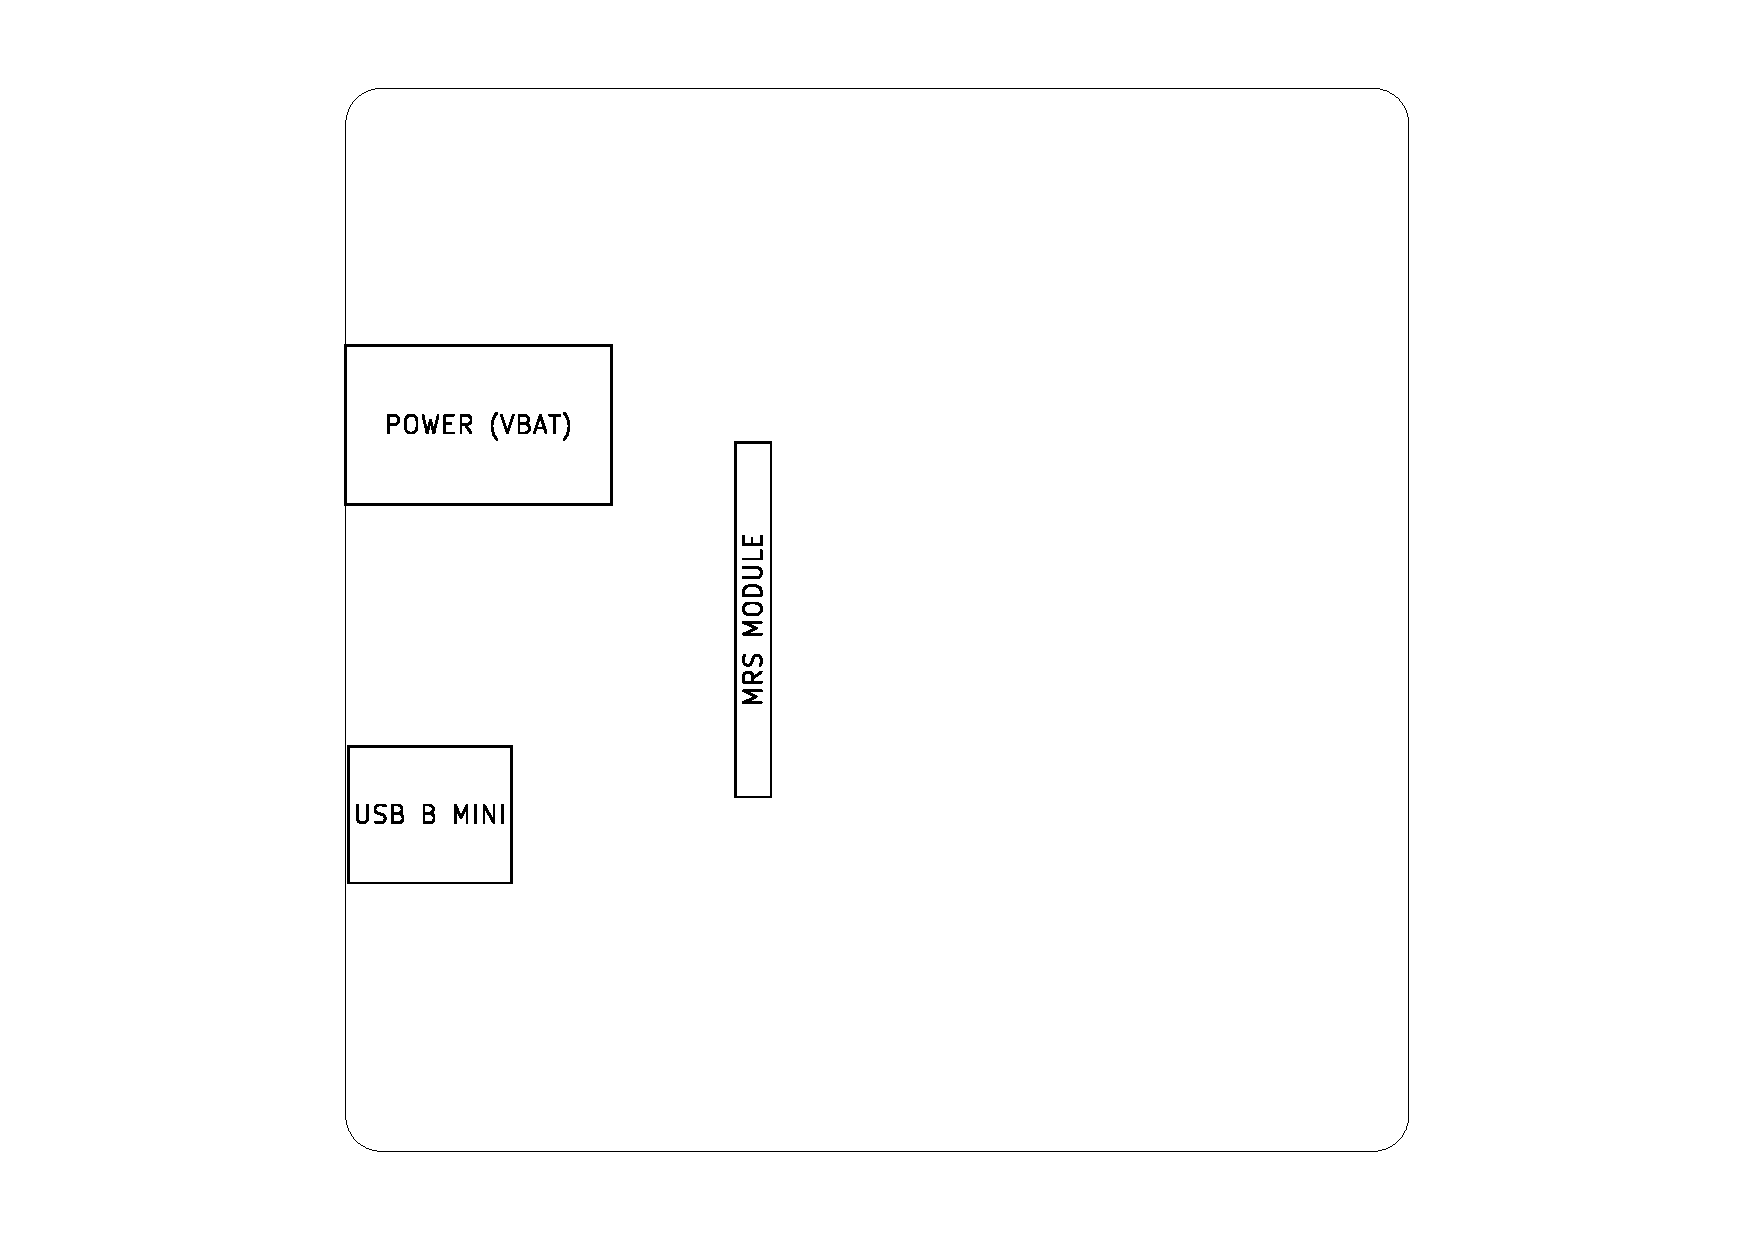
\includegraphics[width=0.7\textwidth]{figures/Connectors_top.pdf}
\caption{MRS MODULE HOST: Connectors Placement, Top Layer}
\label{fig:connectors_top}
\end{figure}

\pagebreak
\newgeometry{left=1cm,right=1cm}
\section{Bill Of Materials and Assembly Drawings}
\begin{longtable}{|p{0.5cm}|p{5cm}|p{5cm}|p{5cm}|p{1.7cm}|}
\hline
\textbf{\#} & \textbf{References}                                                          & \textbf{Value} & \textbf{Footprint} & \textbf{Quantity} 		\\ \hline
1 & C1       & 10uF               & 0603 & 1      				\\ \hline
2 & C2, C3   & 0.1uF              & 0603 & 2                	\\ \hline
3 & J1       & USB2.0B\_mini      & USB\_Mini-B   & 1       	\\ \hline
4 & J2       & Barrel\_Jack       & ADC-028-2-TR   & 1      	\\ \hline
5 & LD1, LD2 & D\_LED\_0603\_BLUE & 0603 & 2                	\\ \hline
6 & MODULE1  & MRS\_Module        & Header 1x10 2mm pitch & 1 	\\ \hline
7 & R1, R2   & 1k                 & R0603 & 2                  	\\ \hline
8 & U1       & FT232RQ            & QFN\_32-5x5mm & 1     	  	\\ \hline
\caption{MRS MODULE HOST: Bill Of Materials}
\label{tab:bom}
\end{longtable}
\vfill
\restoregeometry

\pagebreak
% change scale and angle accordingly
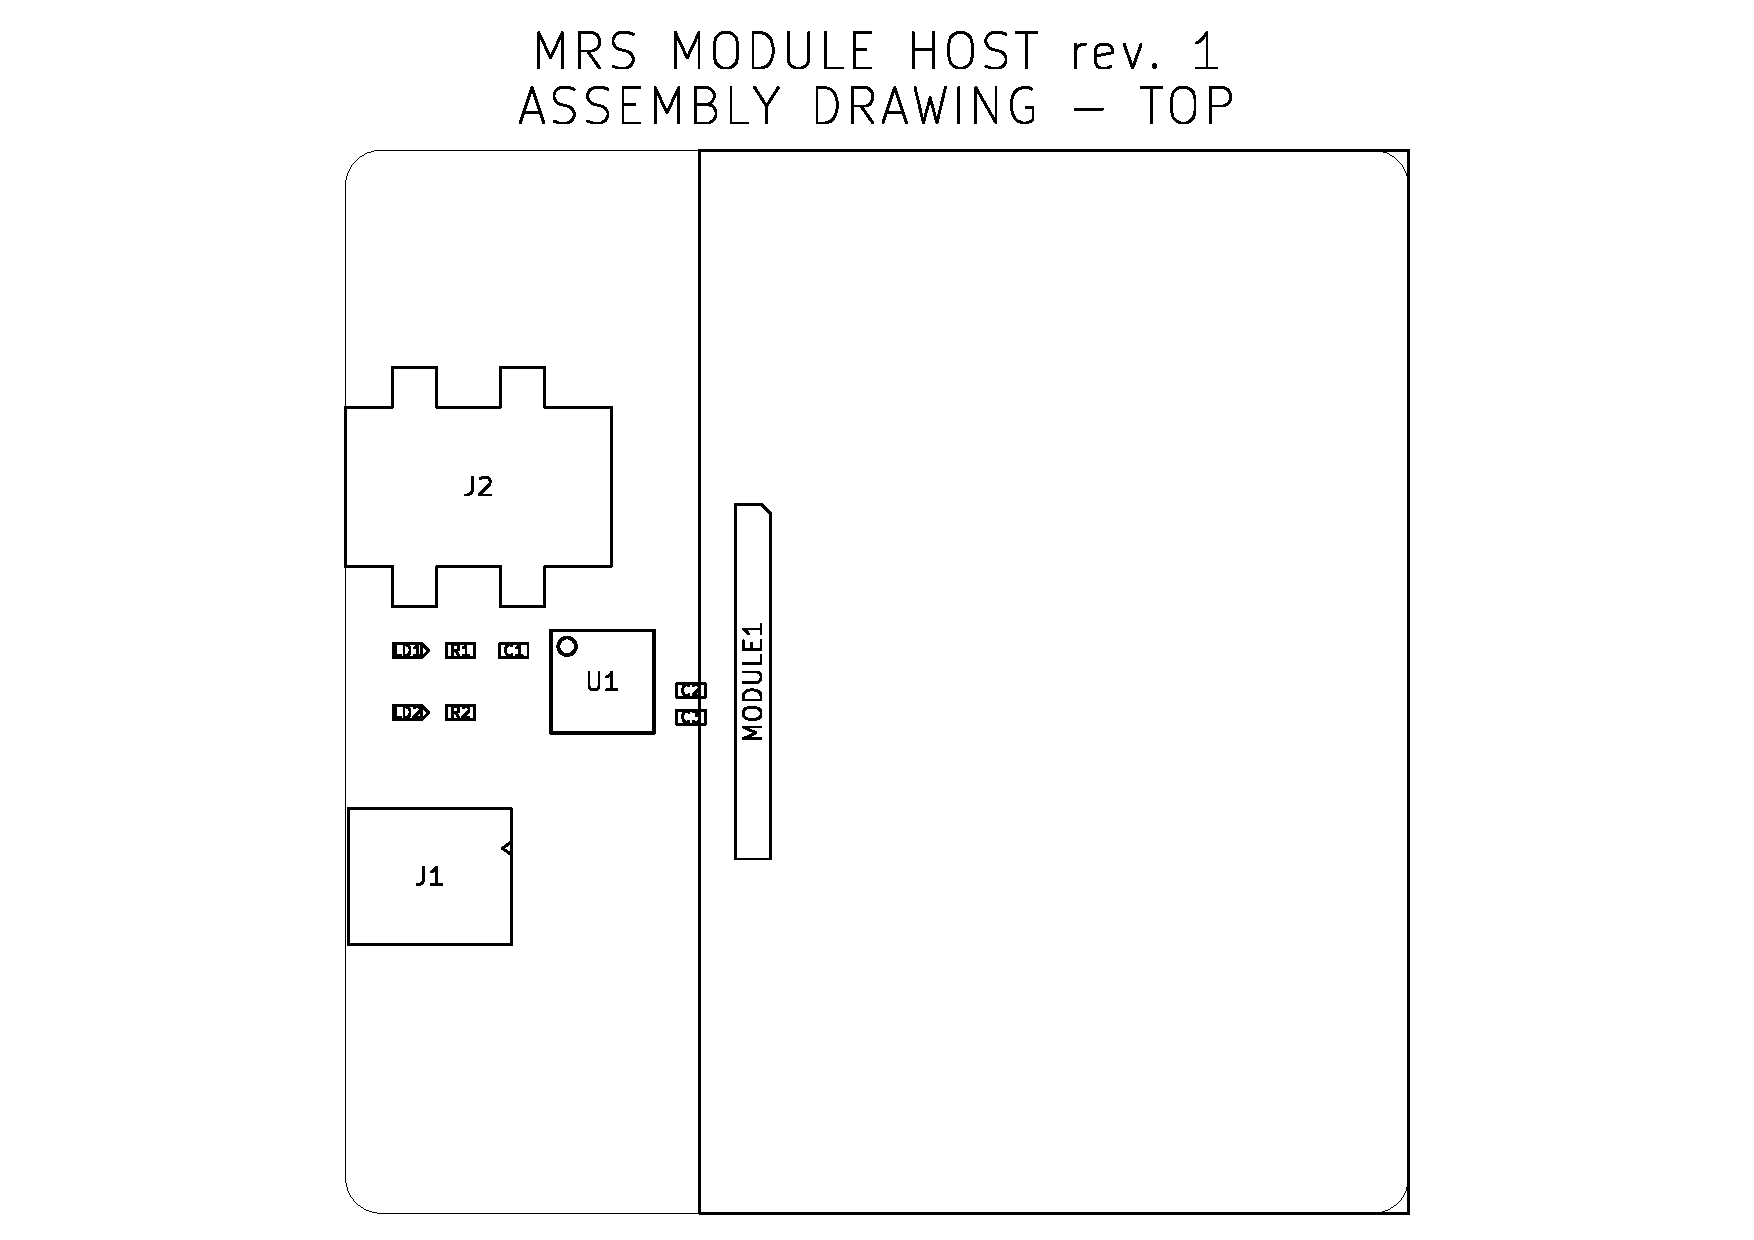
\includepdf[pages=-, scale=1.25, angle=0, pagecommand={}]{figures/Assembly_top.pdf}


\pagebreak
\section{Schematic}
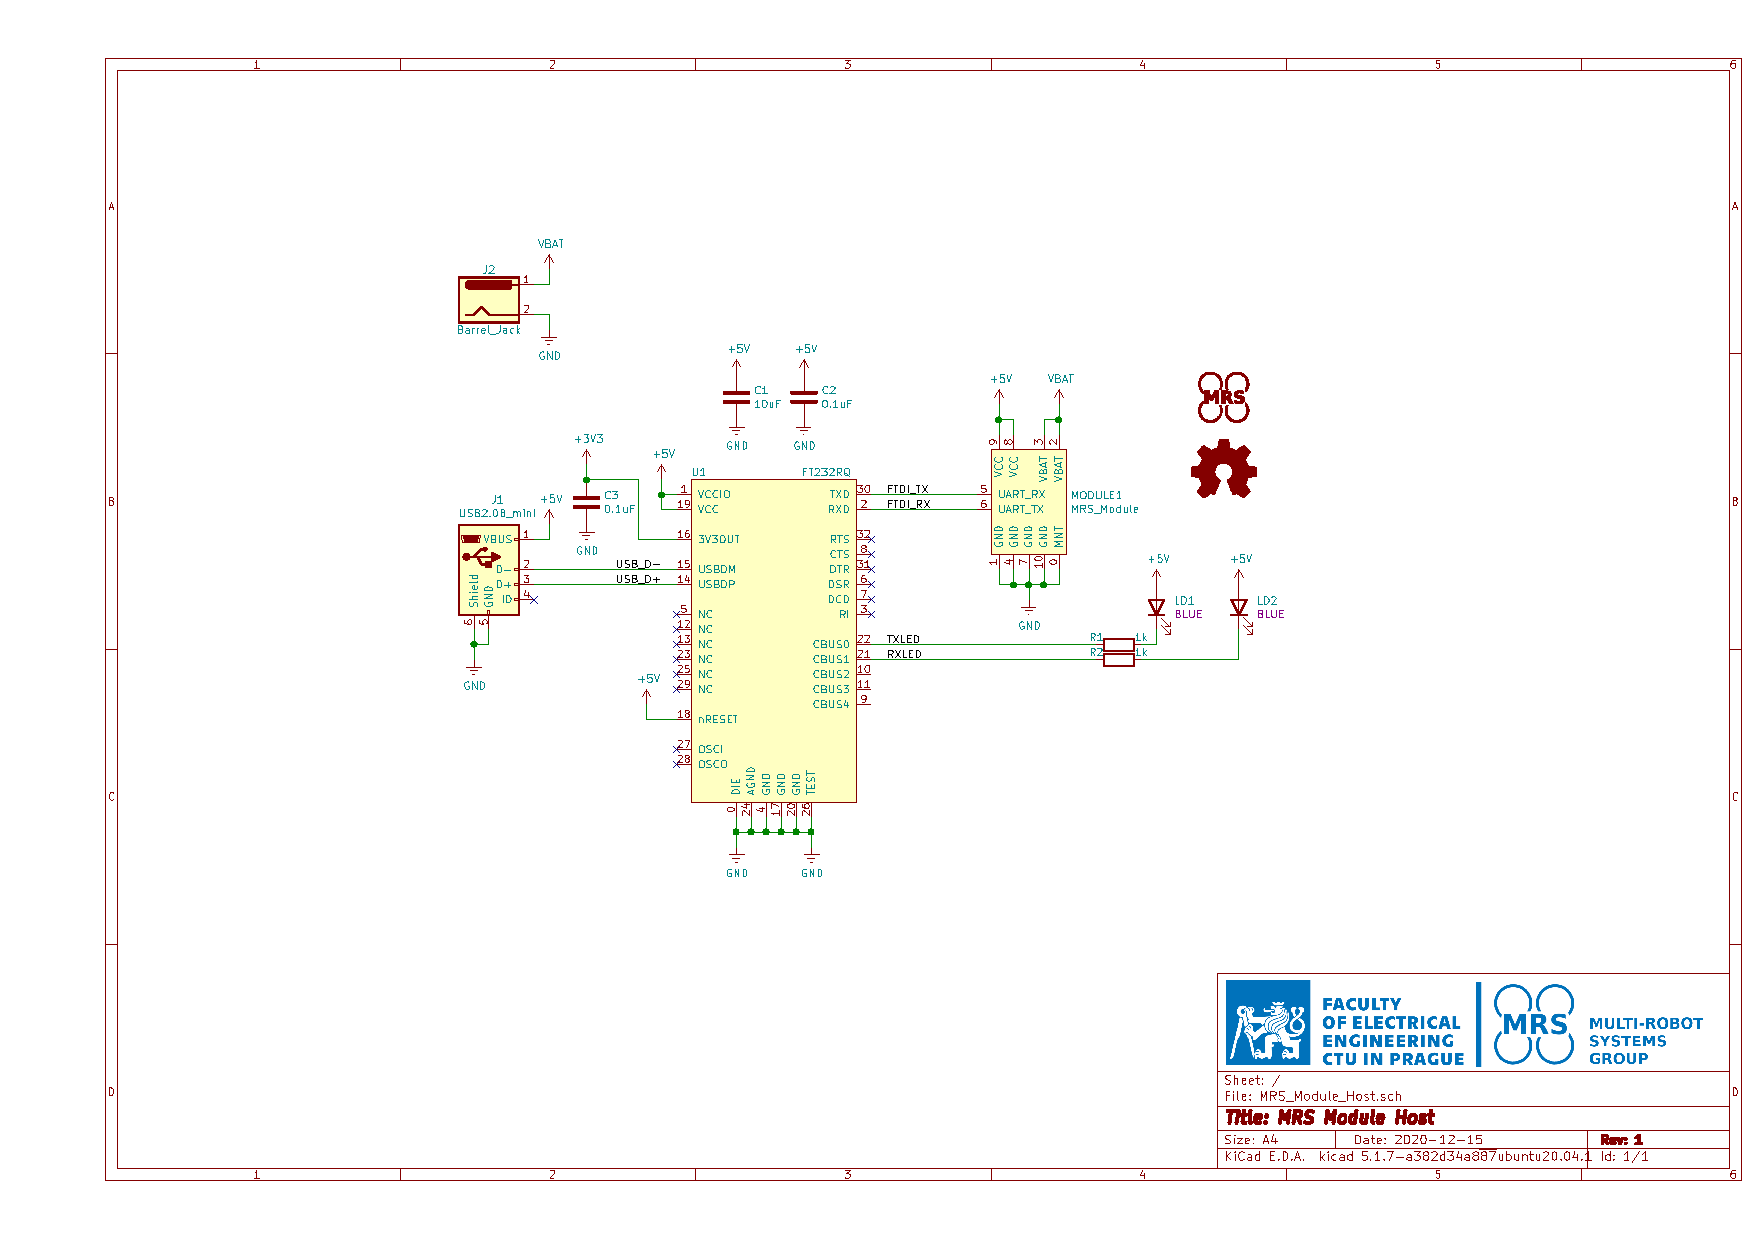
\includegraphics[scale=0.8, angle=270]{figures/Schematic.pdf}

\end{document}